\chapter{Experimental work and result in mixed mode}
\label{Chapter2}

\section{Introduction}

In this section, the results obtained in mixed mode are presented. The decoupling of the modes has allowed to obtain the share of mode 1 and 2. The imposed displacement complacency method has been used to calculate the different energy restitution rates. The deformation maps, force vs crack tip opening curves, energy restitution rate vs crack length for different cases are presented below.It was decided to use only method 1 to measure the crack length as this method appears to be more accurate. The values of the GI/GII ratios and the GI - GII difference are also given. The calculation of the difference is intended to show the behaviour and evolution of the two modes with respect to the variation of alpha.

\section{Experimental set-up and method}

In mixed mode, this camera has the same inclination as the specimen, as shown in Figure \ref{fig:Setup15°}. The crack opening values are therefore projected directly along the x and y axes. The force is projected along the x and y axes, as shown in Figure \ref{fig:fig37bis}.

\begin{figure}[htp]
	\centering
	\includegraphics[width=16cm]{Setup15°}
	\caption{Experimental set-up}
	\label{fig:Setup15°}
\end{figure}

\section{Results}

\subsection{Deformation maps}

Figure \ref{fig:Strain_def_mixedmode} shows the deformation maps for the two tilt angles of the specimen in mixed mode which are $alpha=15°$ and $alpha=30°$. Indeed, we did not have enough specimens to obtain results with $\alpha=45°$.These maps are given in terms of x (pixels) and y (pixels) coordinates. On these different deformation maps, we can clearly see the progression of the crack. The crack propagation path, although not perfectly straight, does not appear to change direction. As in Chapter 3, cracks tend to propagate according to the orientation and inclination of the fibres.

\begin{figure}[htp]
	\centering
	\begin{tabular}{c}
		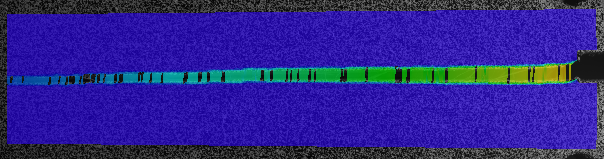
\includegraphics[width=8cm]{e15e2} \\
		e15e2 deformation map \\
		\\
		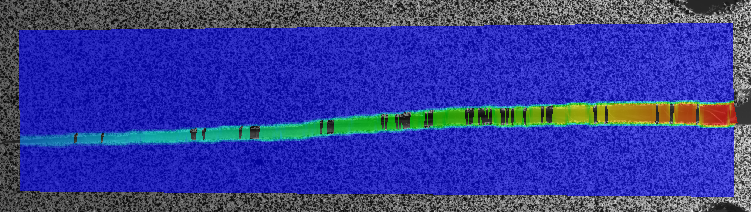
\includegraphics[width=8cm]{e30e3} \\
		e30e3 deformation map \\
		\\
		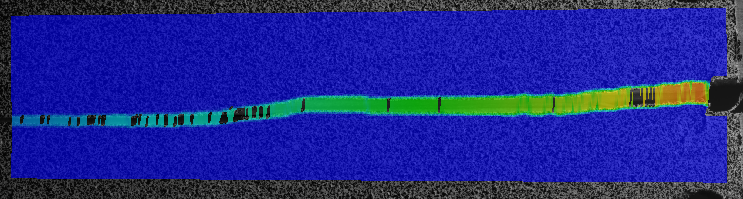
\includegraphics[width=8cm]{e30e5} \\
		e30e5 deformation map \\
	\end{tabular}
	\caption{Typical deformation map ($\epsilon$yy) obtained with DIC for mixed mode}
	\label{fig:Strain_def_mixedmode}
\end{figure}

As in the previous chapter, some curves are verified using deformation maps. Indeed, it is possible to read the crack tip graphically  on the deformation maps. Figure \ref{fig:e15e1_graphicread} and \ref{fig:e30e2_graphicread} show e15e1 and e30e2 verified by graphic reading. It seems that the crack length has been correctly estimated for each satge.

\begin{figure}[htp]
	\begin{minipage}[c]{.46\linewidth}
		\centering
		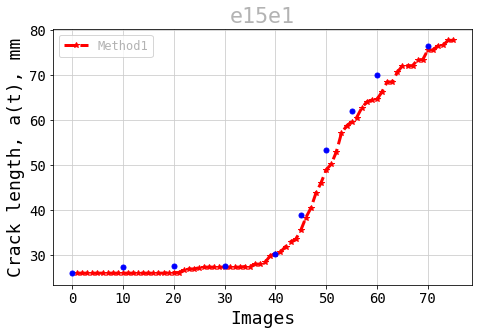
\includegraphics[width=8cm]{e15e1_graphicread}
		\caption{Crack tip by graphic reading e15e1}
		\label{fig:e15e1_graphicread}
	\end{minipage}
	\hfill%
	\begin{minipage}[c]{.46\linewidth}
		\centering
		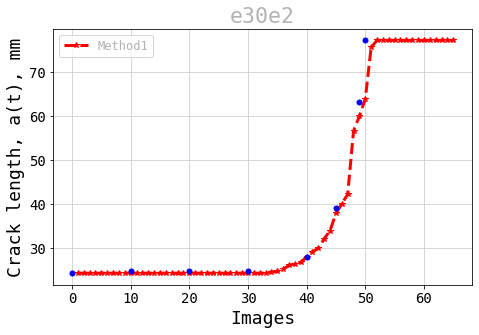
\includegraphics[width=8cm]{e30e2_graphicread}
		\caption{Crack tip by graphic reading e30e2 }
		\label{fig:e30e2_graphicread}
	\end{minipage}
\end{figure}

\subsection{Force - Crack Tip Opening Curve}

Figure \ref{fig:CTOD15} shows the evolution of the force as a function of the crack tip opening for $\alpha=15°$. For all the specimens, when a sudden drop in P is observed, signifying the complete failure of the material, the values along the x axis are less than 0.15 mm and of the order of 0.5 to 1.1 mm along the y axis.

\begin{figure}[H]
	\centering
	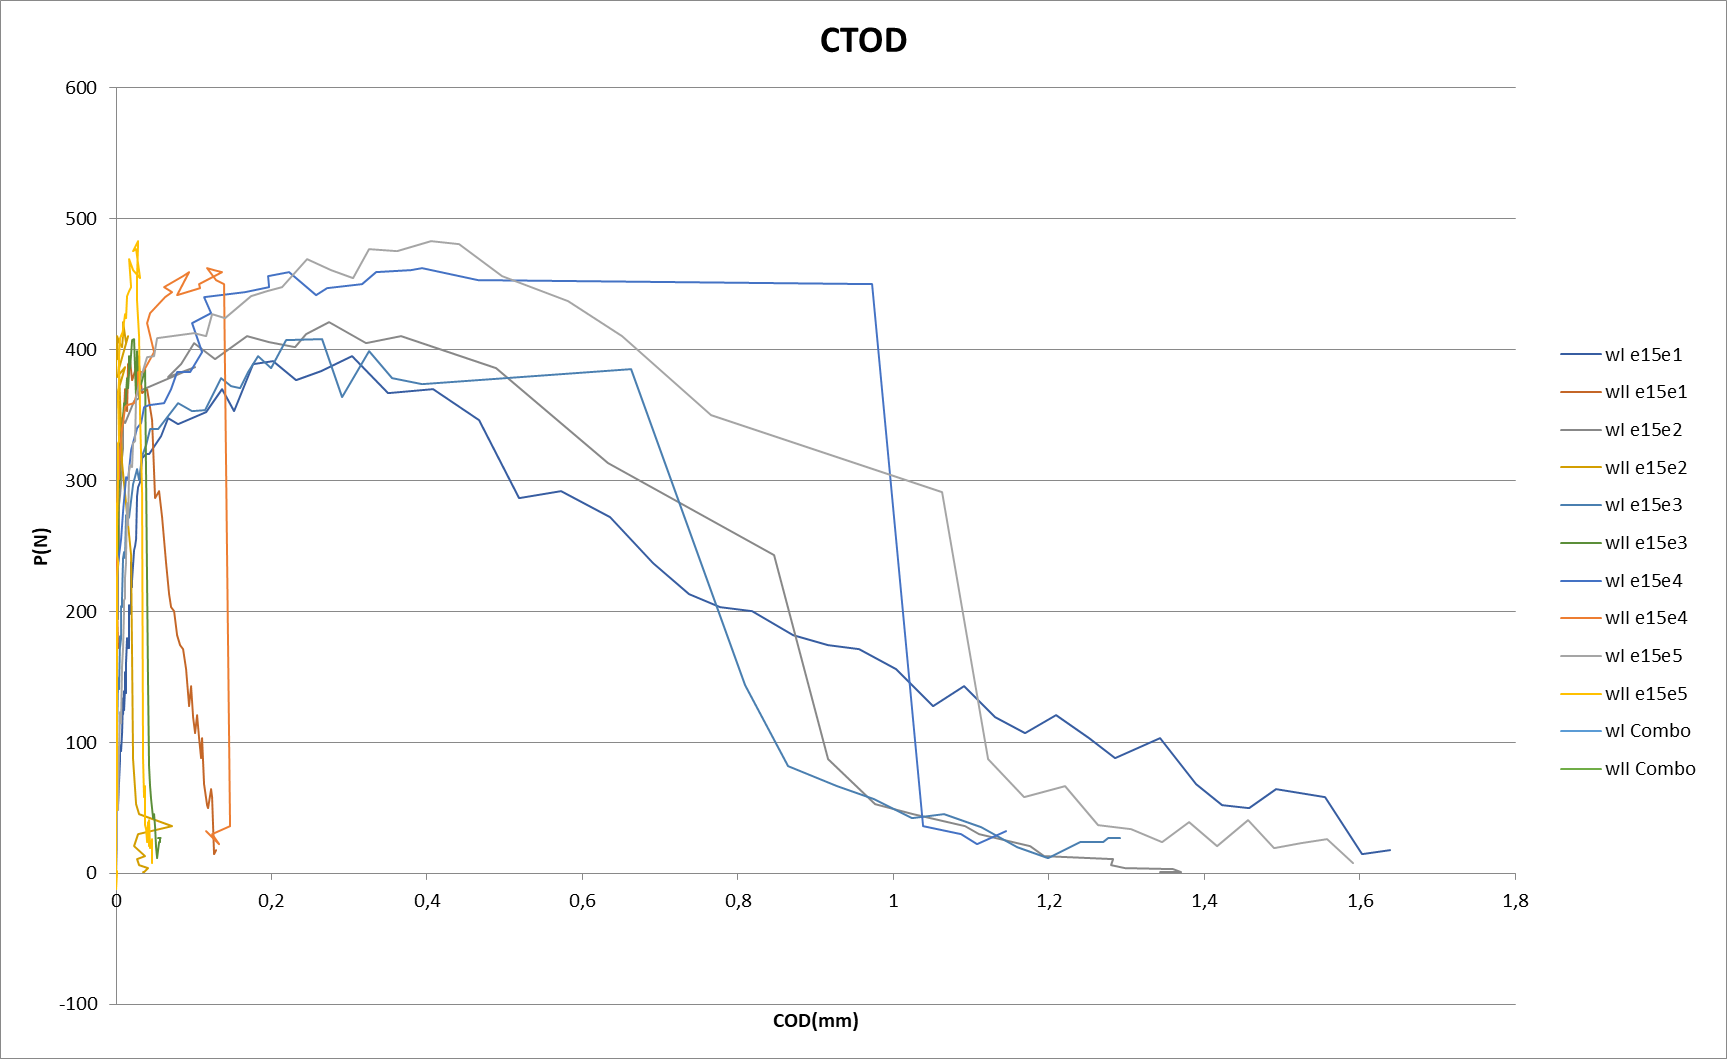
\includegraphics[width=16cm]{CTOD15}
	\caption{Evolution of the force as a function of the crack opening for $\alpha=15°$}
	\label{fig:CTOD15}
\end{figure}

Figure \ref{fig:CTOD30} shows the force curves as a function of the crack opening for $\alpha=30°$. As can be seen, the crack opening along x for all the specimens tested is less than 0.11 mm. For the crack opening along y when a sudden drop in P is observed, the values are of the order of 0.3 to 1.1 mm. 
We can also see that the CTOD of e30e2 does not have the expected shape. After the image 53 of 66, the CTOD is not recorded correctly. However, this is of no real importance as P decreases sharply at stage 49, so it has no impact on the calculation of Gmax.

\begin{figure}[H]
	\centering
	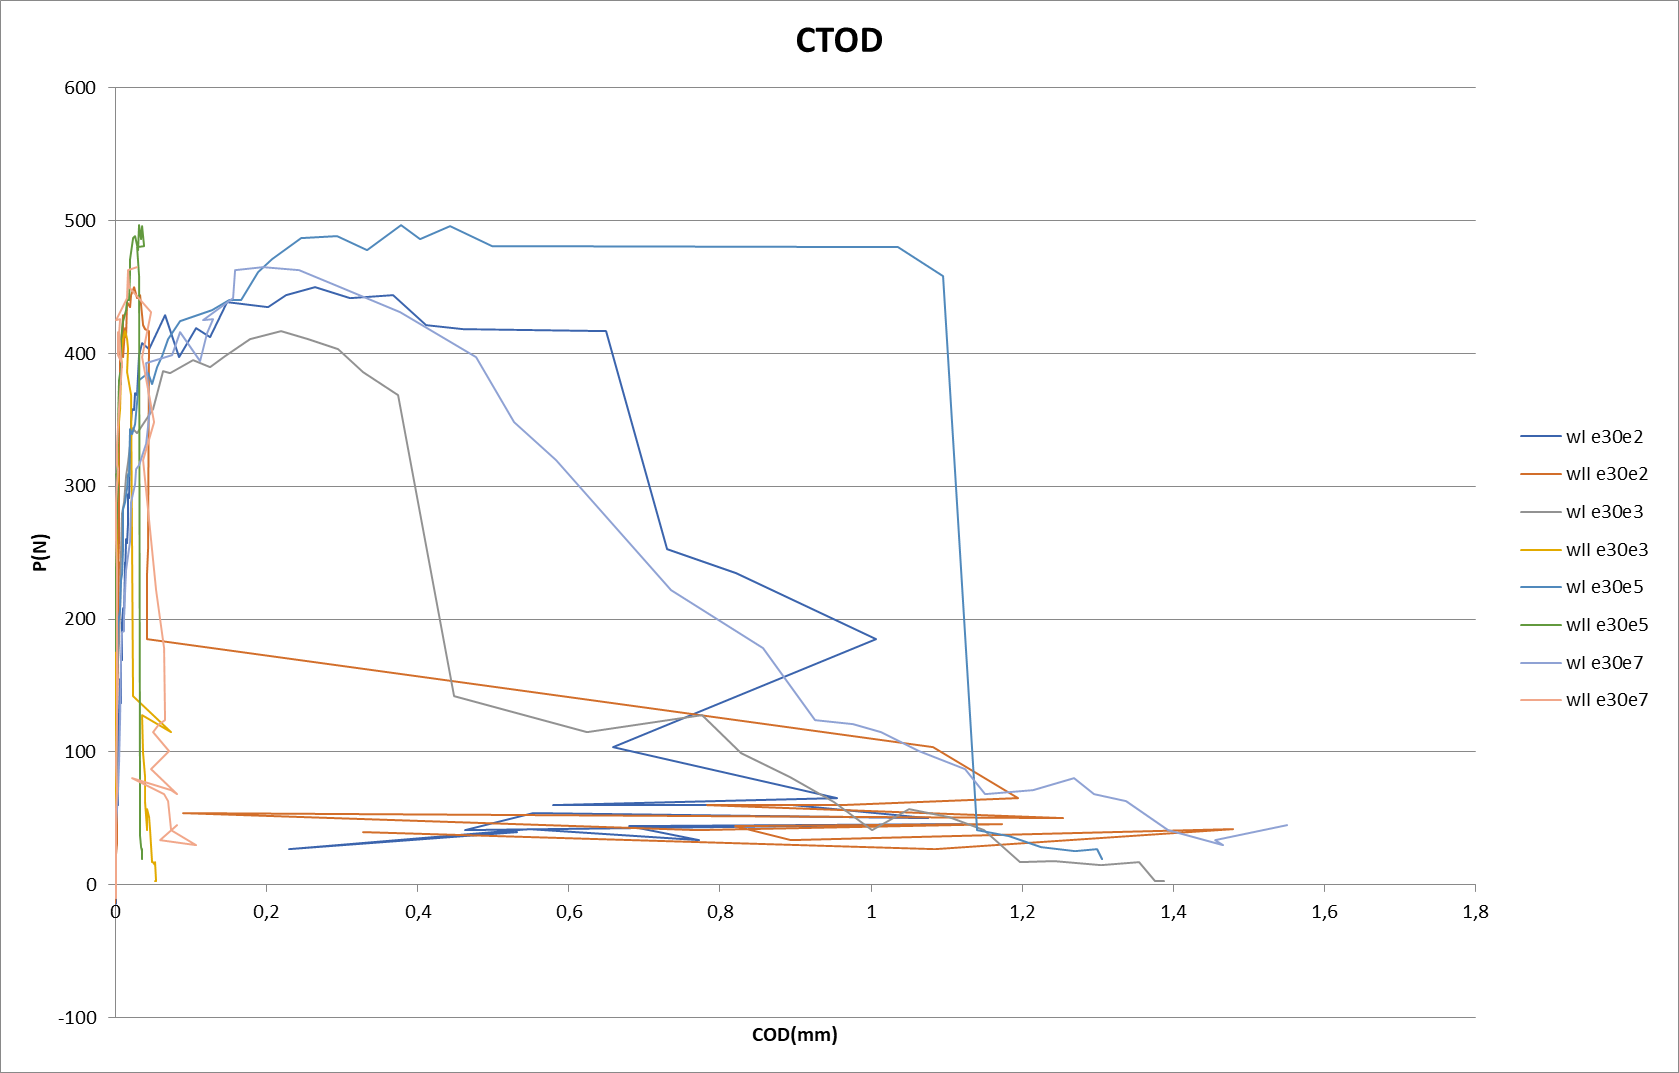
\includegraphics[width=16cm]{CTOD30}
	\caption{Evolution of the force as a function of the crack opening for $\alpha=30°$}
	\label{fig:CTOD30}
\end{figure}

We can say that for $\alpha=15°$ and $\alpha=30°$ the crack openings along the x-axis are negligible compared to those along the y-axis. 

\subsection{Crack length curves}

All the crack length curve in function of displacement in mixed mode are shown in figure \ref{fig:crack_15} and \ref{fig:crack_30} with the method 1. 
There are, as expected, different plateaus for the crack length. The crack length increases gradually and continuously before rupture. It is interesting to examine all the crack length propagation plots.  The curves are all more or less the same shape, and the crack ends at roughly the same length. What differs is the stage at which the crack begins to propagate. There are no major differences in crack length when you switch from mode I to mixed mode.

\begin{figure}[htp]
	\centering
	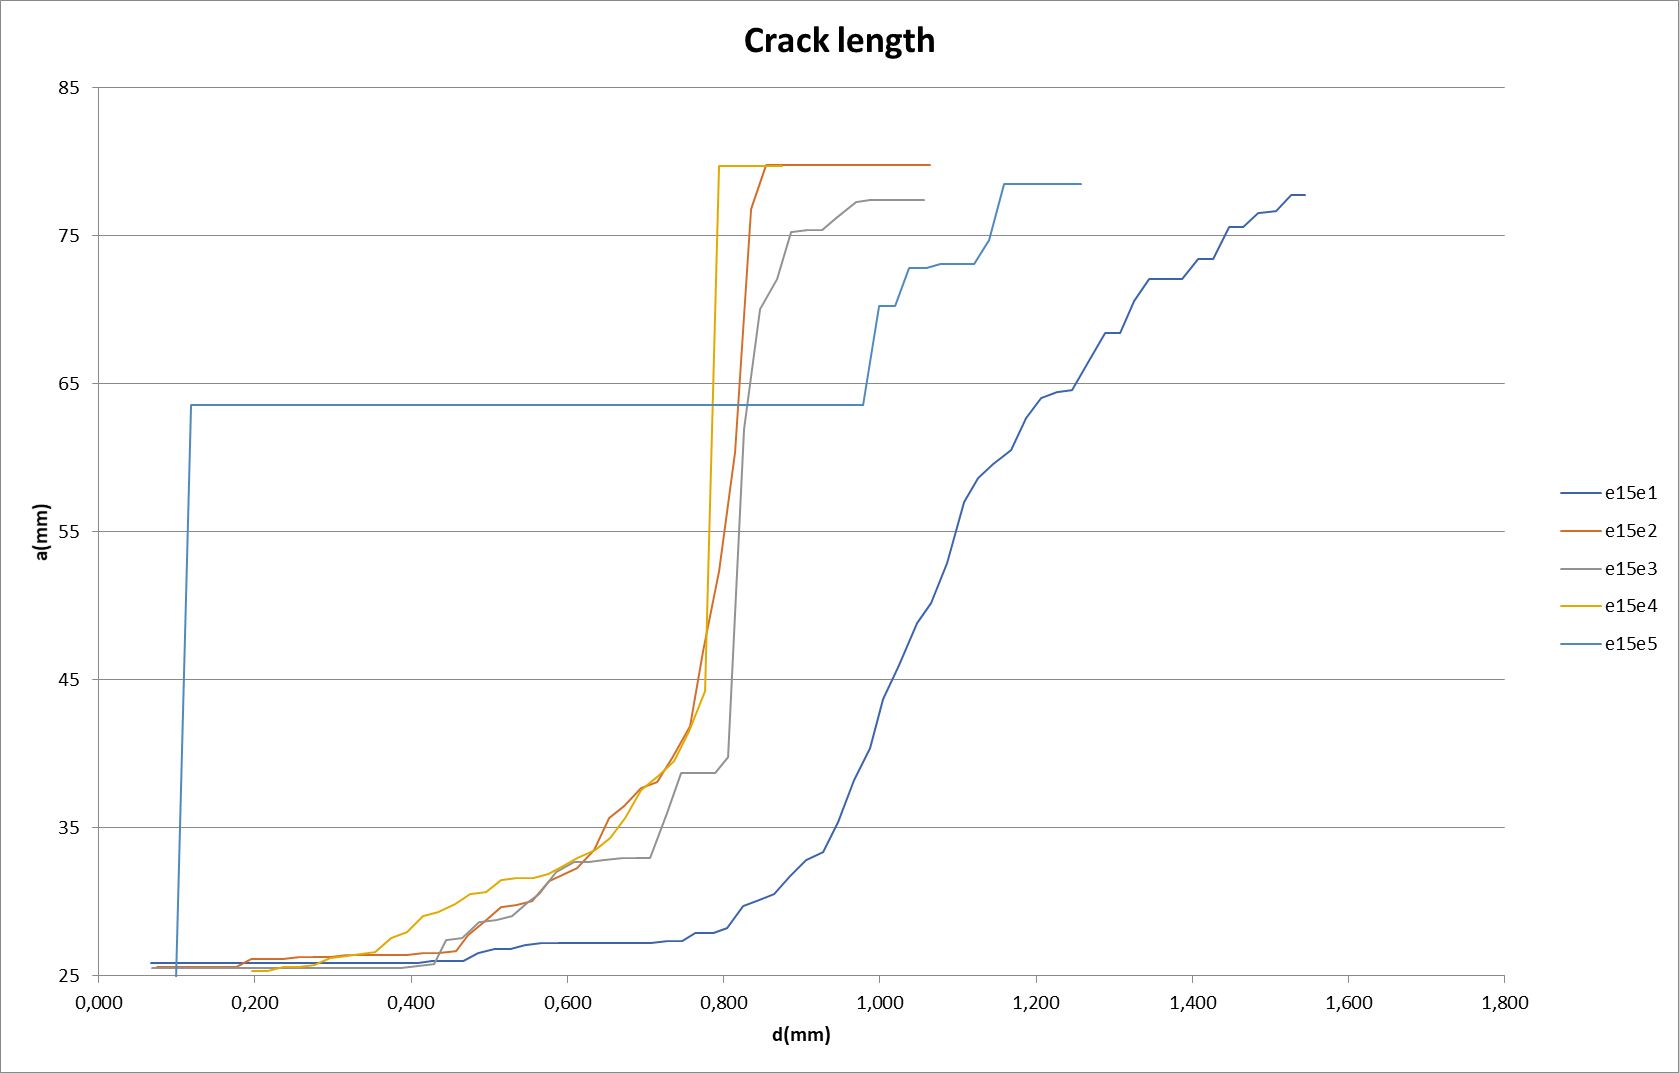
\includegraphics[width=13cm]{crack_15}
	\caption{Crack length evolution for $\alpha=15$}
	\label{fig:crack_15}
\end{figure}

\begin{figure}[htp]
	\centering
	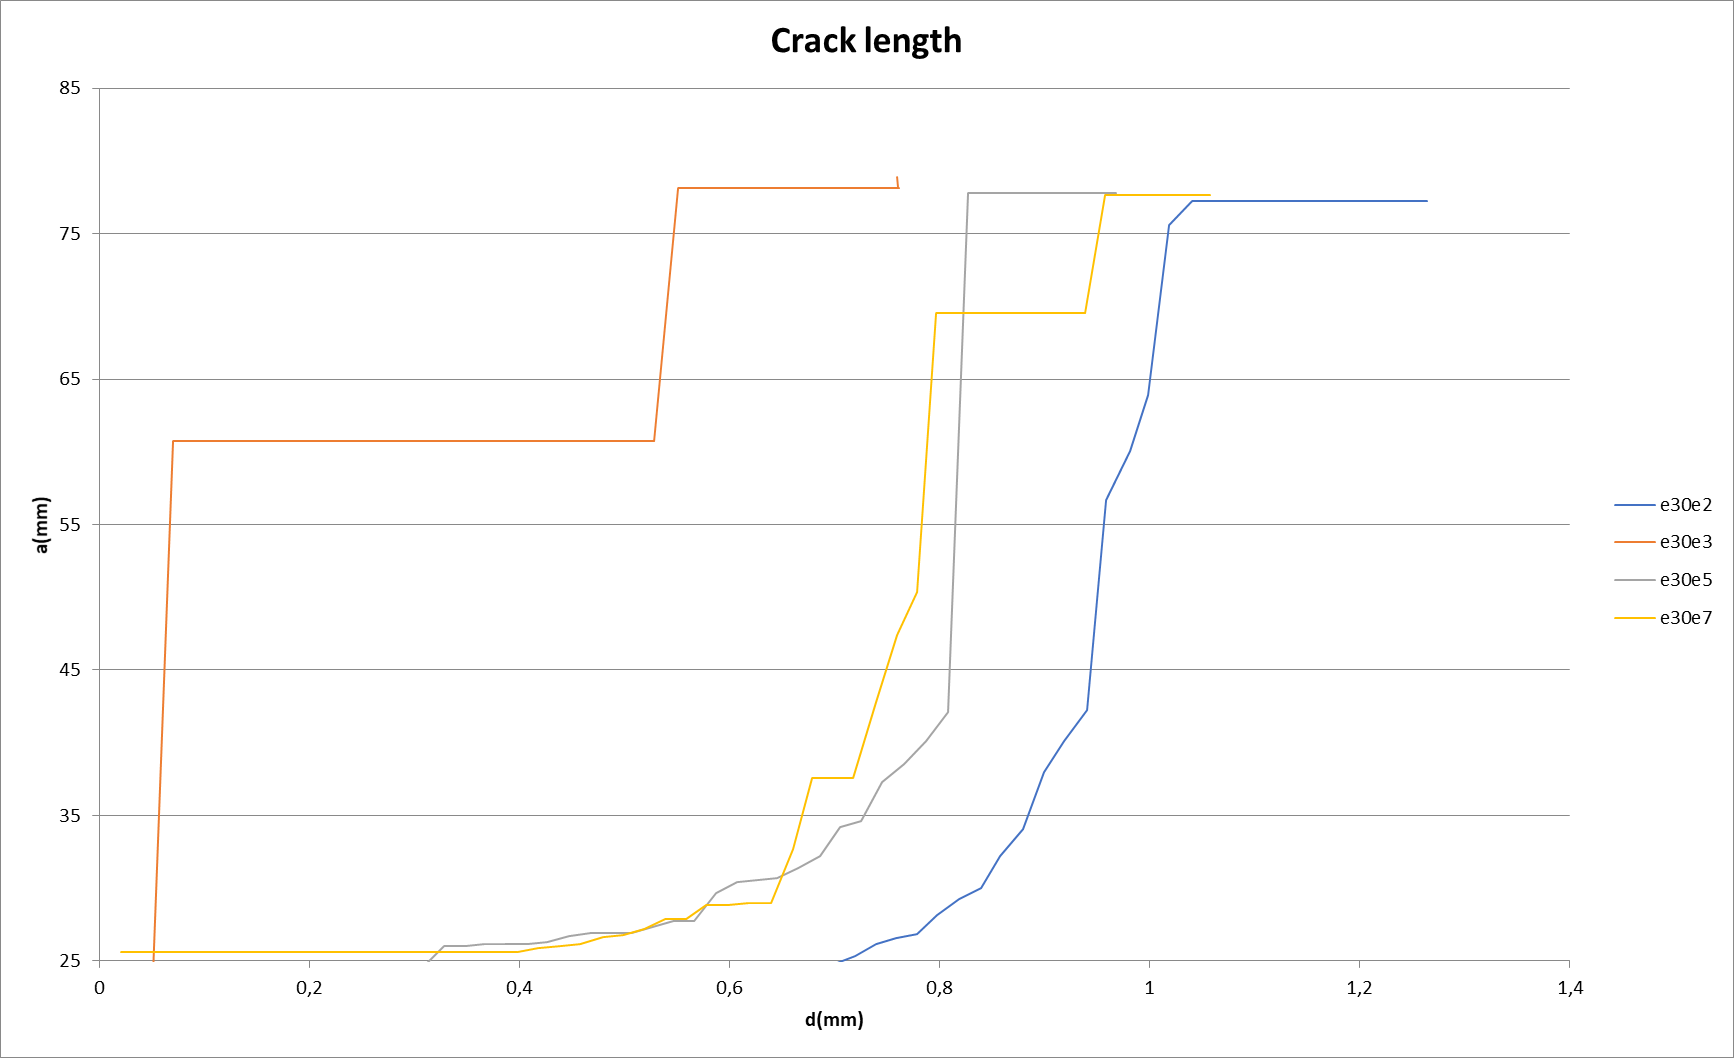
\includegraphics[width=13cm]{crack_30}
	\caption{Crack length evolution for $\alpha=30$}
	\label{fig:crack_30}
\end{figure}

\subsection{Critical energy restitution rate}

\begin{figure}[htp]
	\centering
	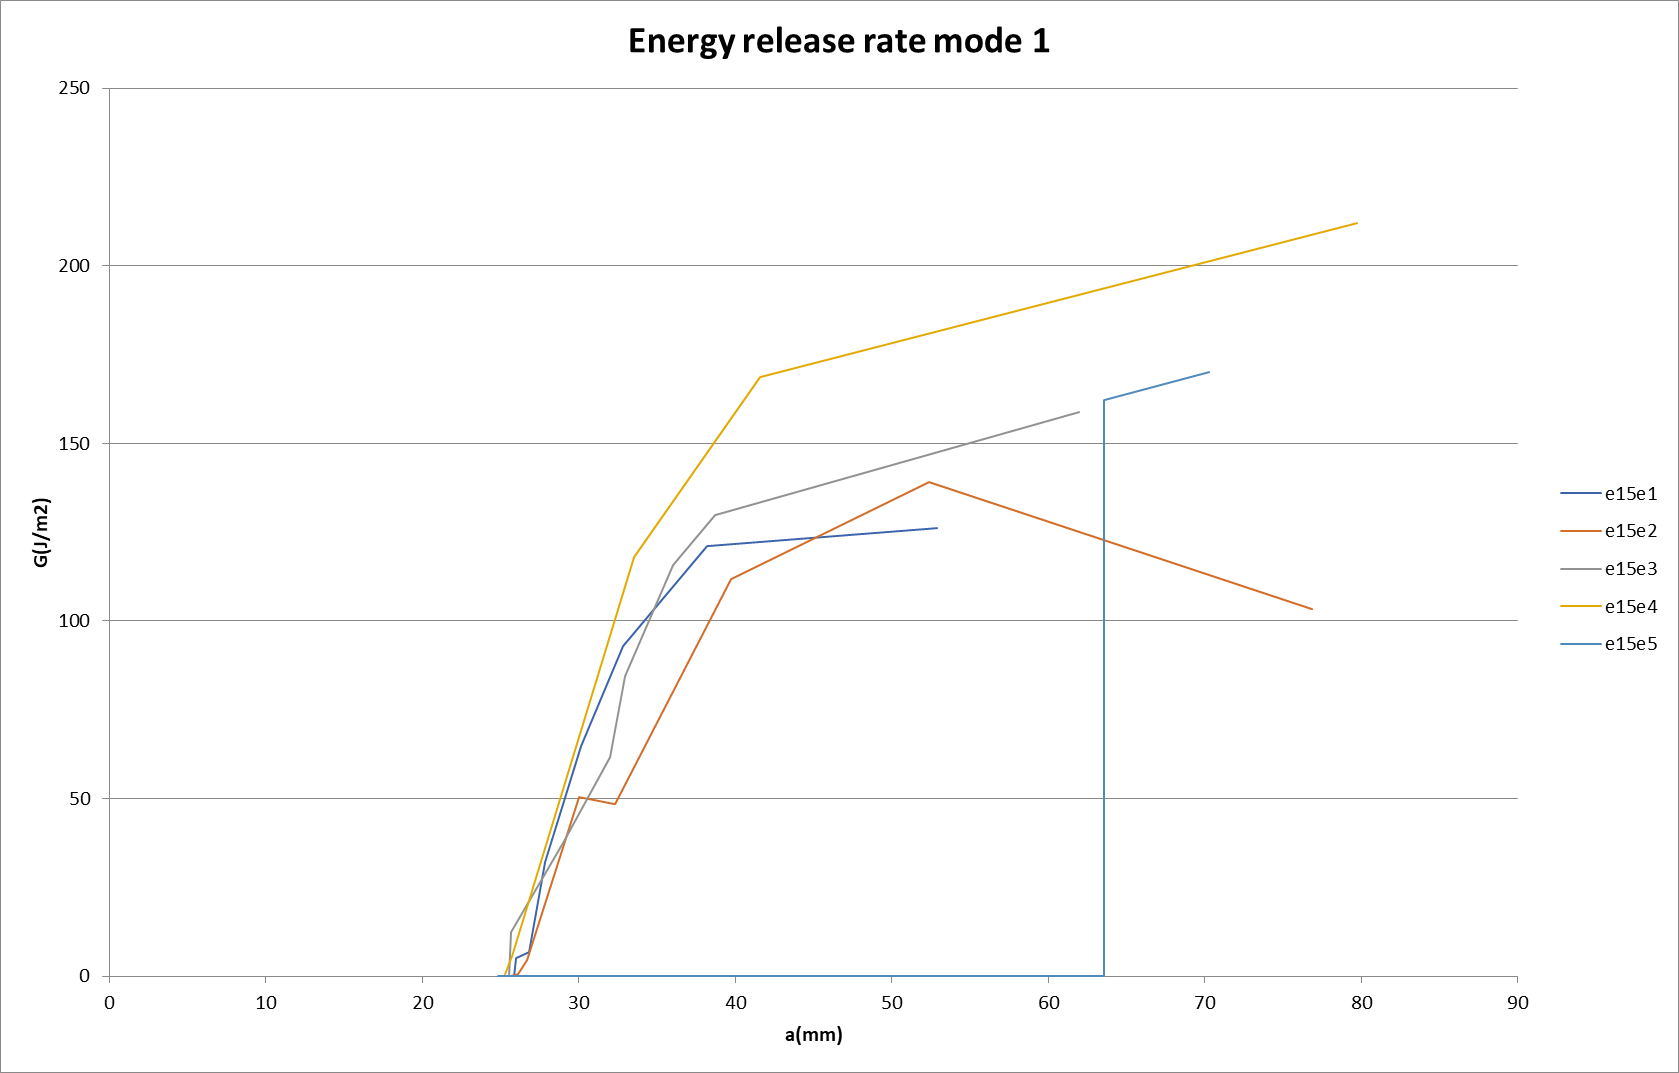
\includegraphics[width=12.5cm]{G1_15}
	\caption{Energy restitution rate as a function of crack length for alpha=15; mode I share}
	\label{fig:G1_15}
\end{figure}

\begin{figure}[htp]
	\centering
	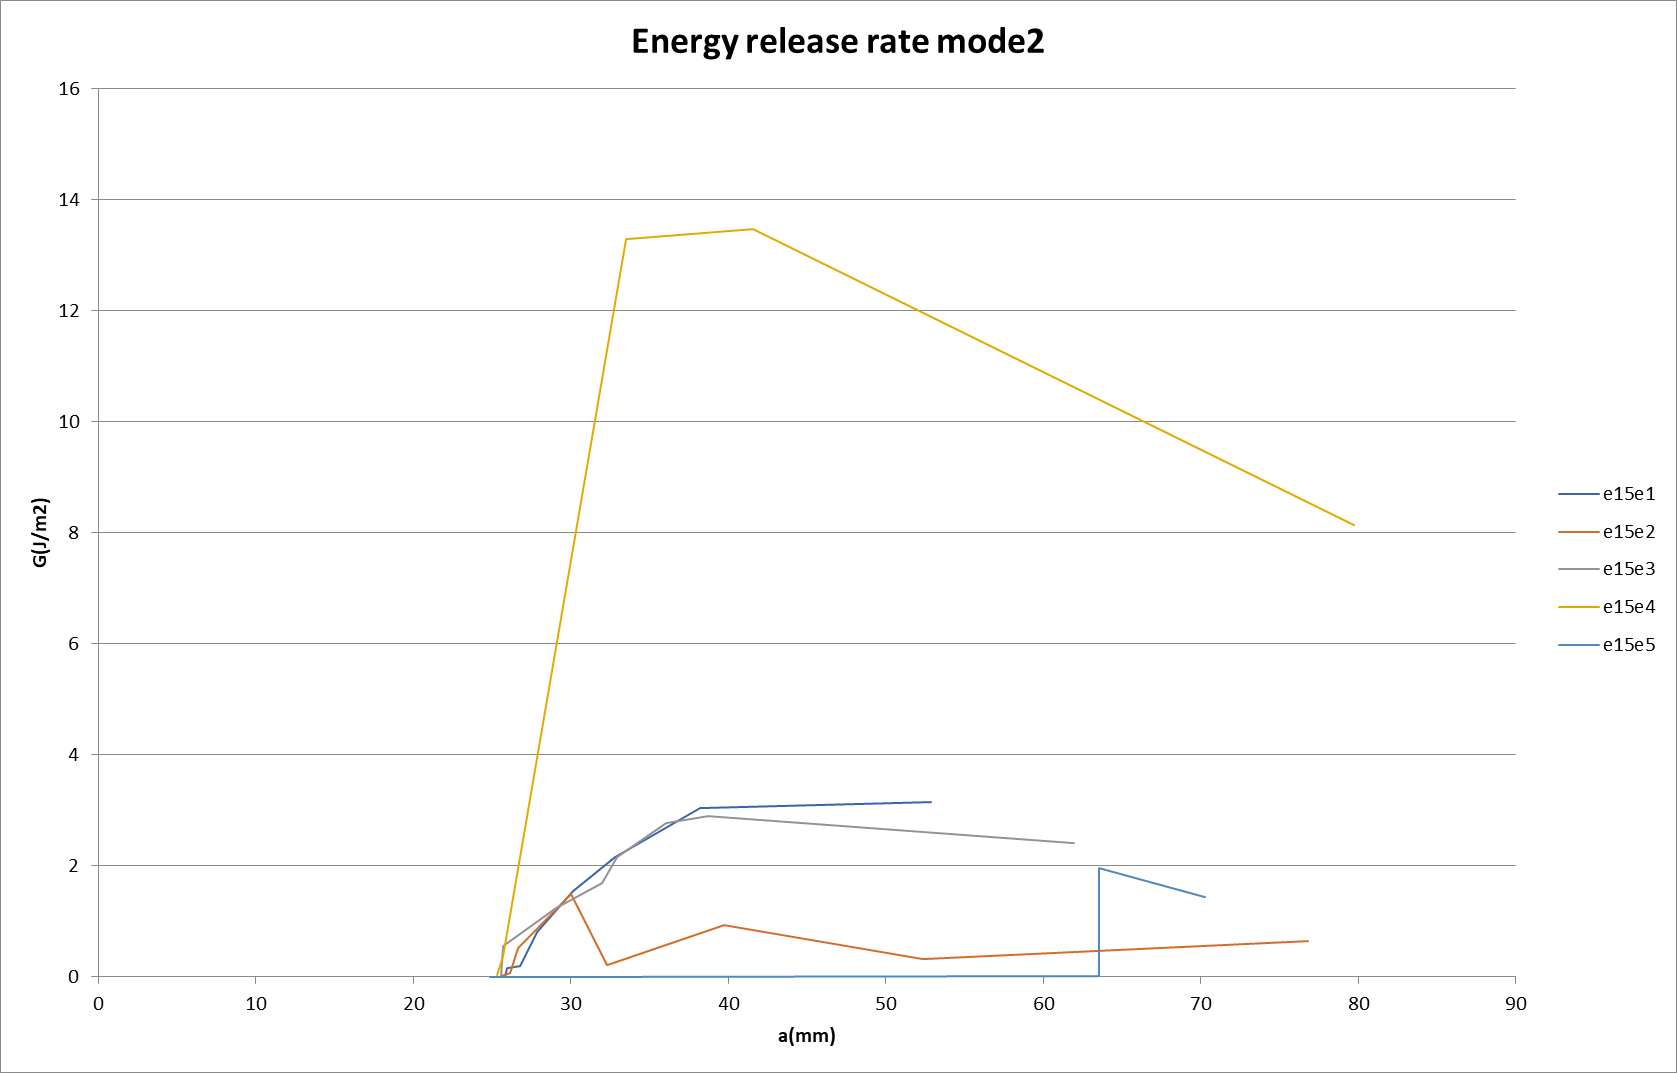
\includegraphics[width=12.5cm]{G2_15}
	\caption{Energy restitution rate as a function of crack length for alpha=15; mode II share}
	\label{fig:G2_15}
\end{figure}

\begin{figure}[htp]
	\centering
	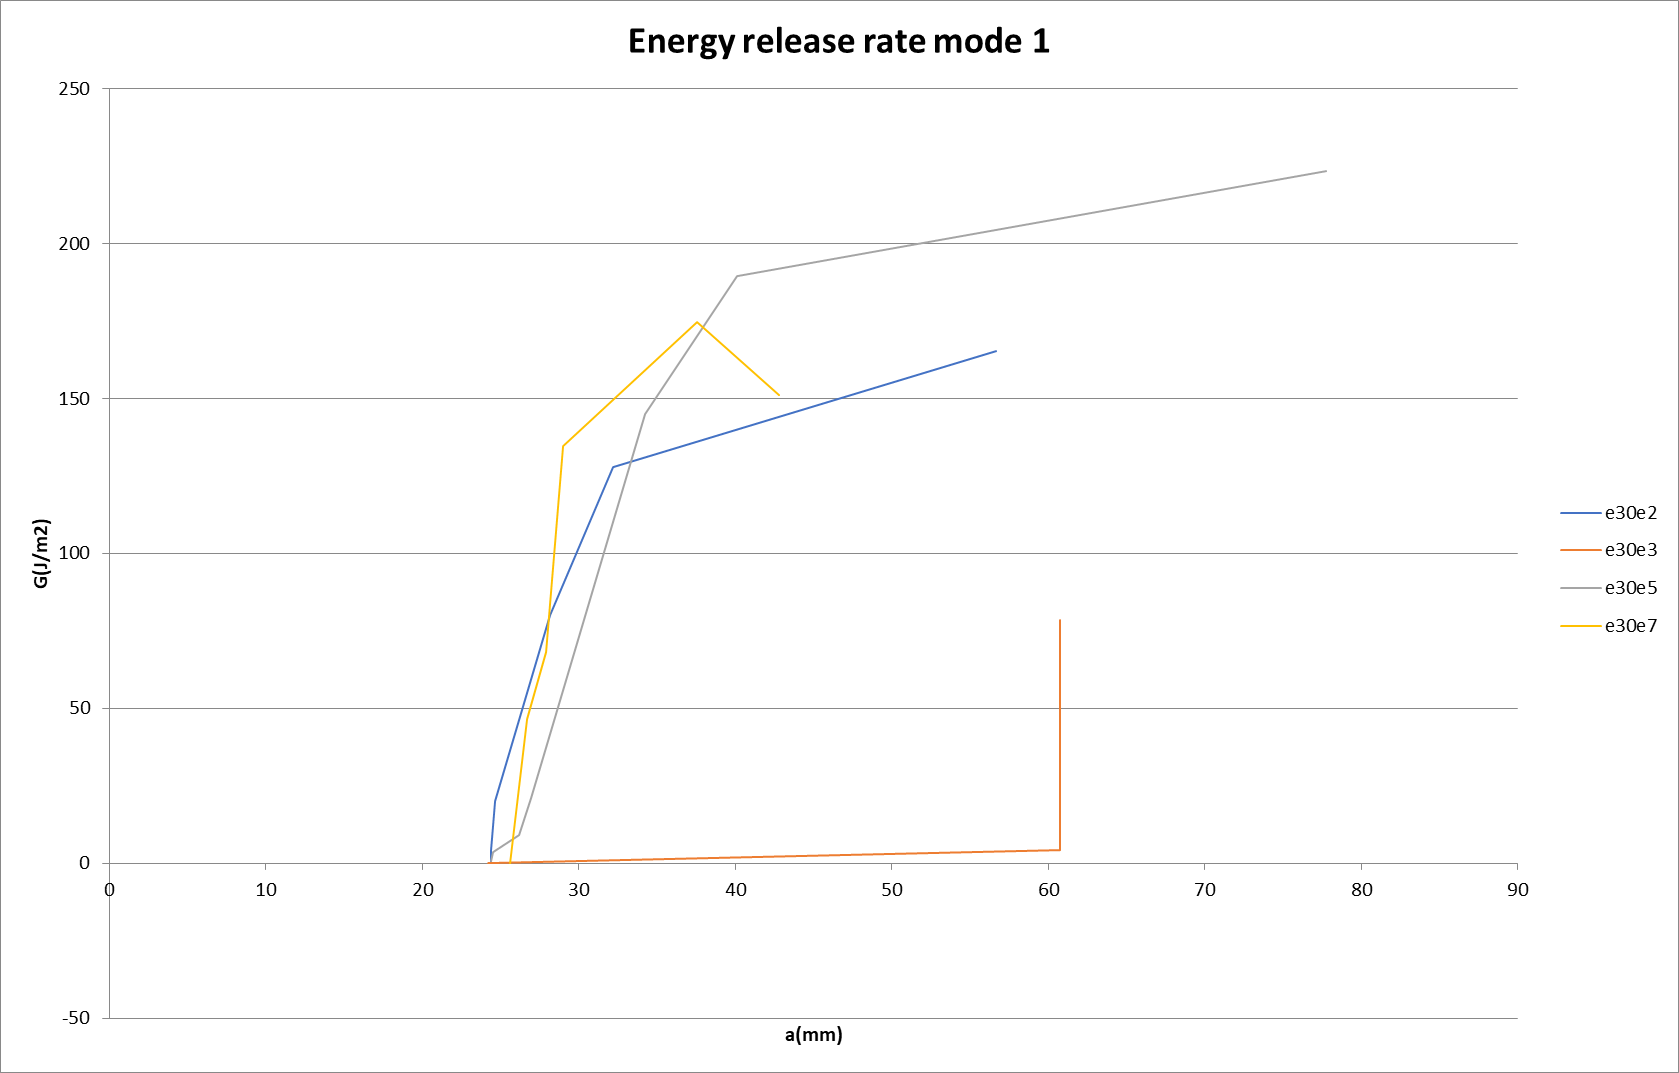
\includegraphics[width=12.5cm]{G1_30}
	\caption{Energy restitution rate as a function of crack length for alpha=30; mode I share}
	\label{fig:G1_30}
\end{figure}

\begin{figure}[htp]
	\centering
	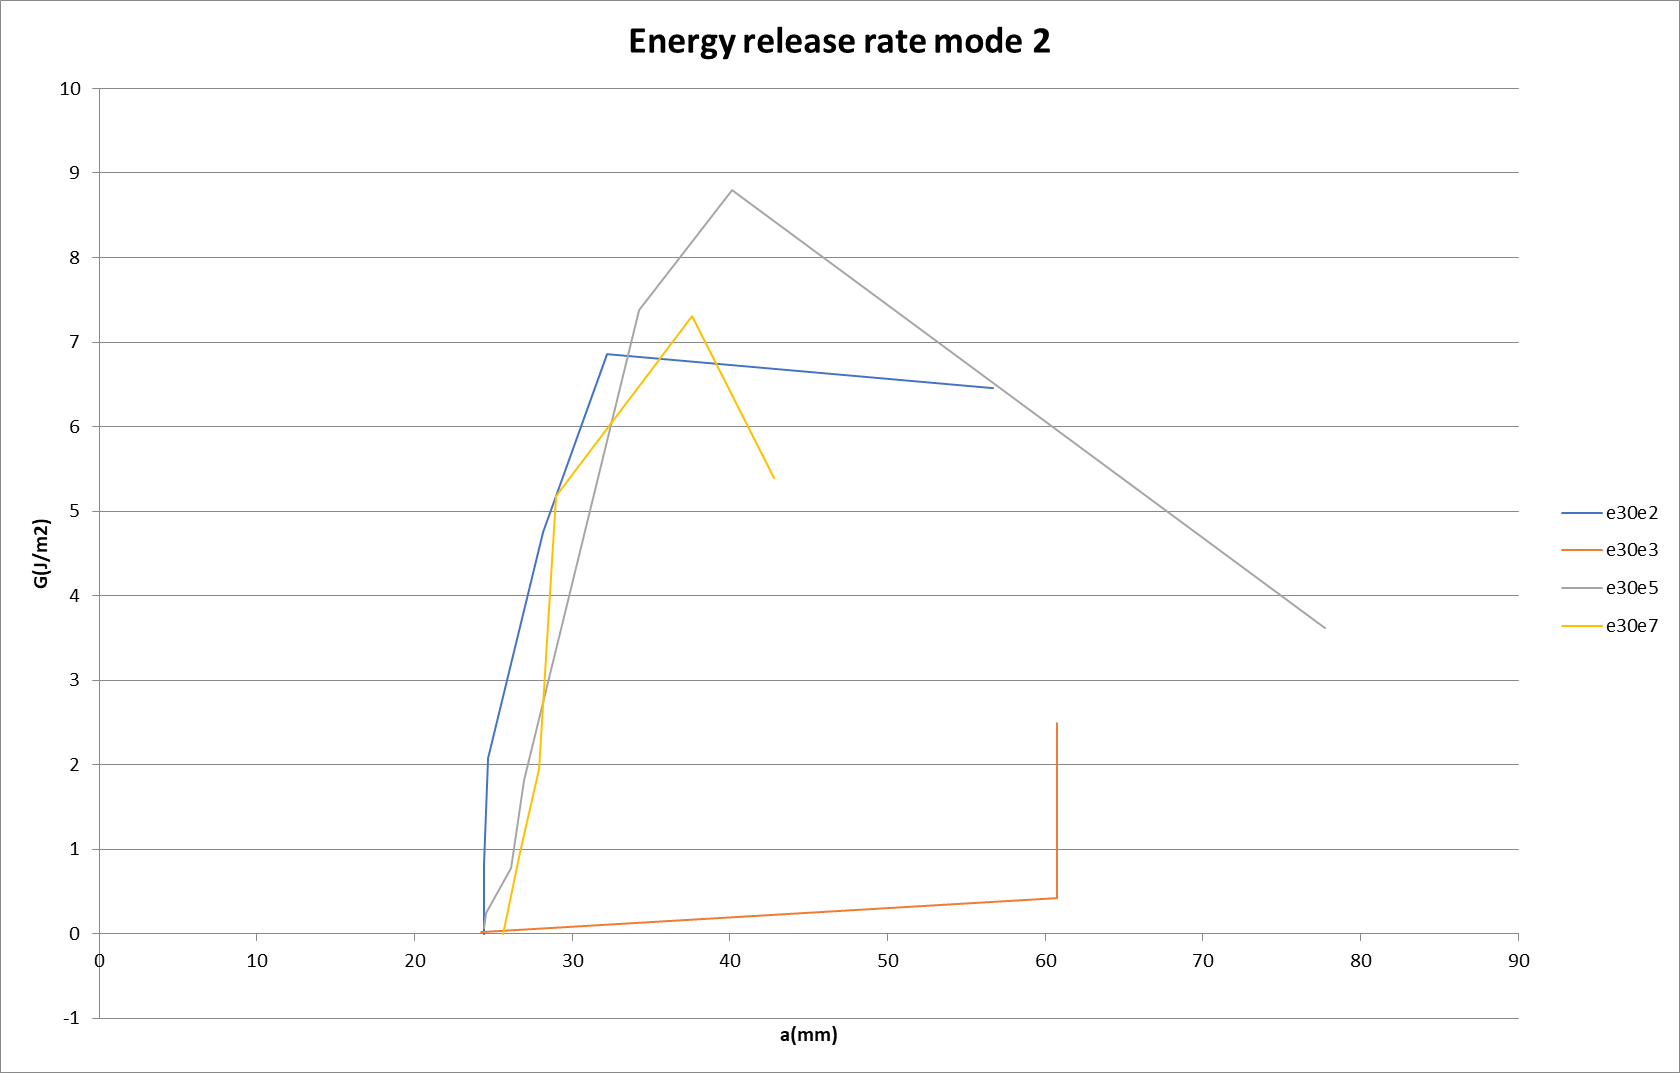
\includegraphics[width=12.5cm]{G2_30}
	\caption{Energy restitution rate as a function of crack length for alpha=30; mode II share}
	\label{fig:G2_30}
\end{figure}

\section{Data analysis and comparisons}

\subsection{Data analysis}

Table x shows the different values of G. The differences in mode 1 and 2 are compared.
Figure x shows the difference in the values of the energy restitution rates GI - GII according to the different mixing angles. We can clearly see the decrease of this difference between the mode 1 and mode 2 share with the increase of the mixing angle.

After analysis of the tests for the different mix ratios, the results obtained gave the following information:

For all the mix angles studied, the mode 1 share is always higher than the mode 2 share

The energy restitution rate values from mode 1 decrease with increasing degree of mixing angle, while the energy restitution rate values from mode 2 increase

The GI/GII ratio as a function of crack length has a constant evolution as shown in Figure x. This may indicate that the values characterising the cracking obtained are intrinsic to the species studied

The difference between the GI-GII values decreases with increasing degree of the mixing angle (Figure x) justifying at the same time the complete decoupling of the mixed modes of failure. In figure x, the results of the GI-GII values obtained for the tests with an angle of 15, 30 and 45 degrees are shown. We can see a decreasing evolution of this difference. This can be explained by the fact that when we approach an angle of 45 degrees, the values of the crack openings along x and y tend to get closer. In mixed mode, the crack opening is no longer one-dimensional since the specimen is stressed at an angle that induces the cohabitation of two modes, which leads to a projection along both axes of the crack opening. Obtaining the two components Ux and Uy led to the calculation of GI and GII . In other words, this allows the decoupling of the two modes. The difference between the values of the two modes is therefore maximal when the mixing angle is 15 degrees . It will decrease until the angle of 45 degrees where it is minimal. Between 0 degrees and 45 degrees mode 1 is superior to mode 2. It is probably after a mixing angle of 45 degrees that mode 2 is supposed to be superior to mode 1.

\subsection{Difficulties and way of amelioration}

Figure \ref{fig:Crack_junction} shows the MMCG specimen with cracks at the connection fillet. Indeed, among the difficulties encountered, the brittleness of the specimens at the level of the connection fillet is precisely the one that caused the most problems. It is for this reason that several tests were not used. 3 tests with a 30° angle and one test with a 45° angle broke at the connection fillet. 1 specimen at 0° did not crack at the initial crack tip and finally one specimen broke because the machine stopped abruptly during the test because it was overheating. In conclusion, 14 tests were successful and it was only possible to analyse for the 0, 15 and 30 degree angles.

\begin{figure}[htp]
	\centering
	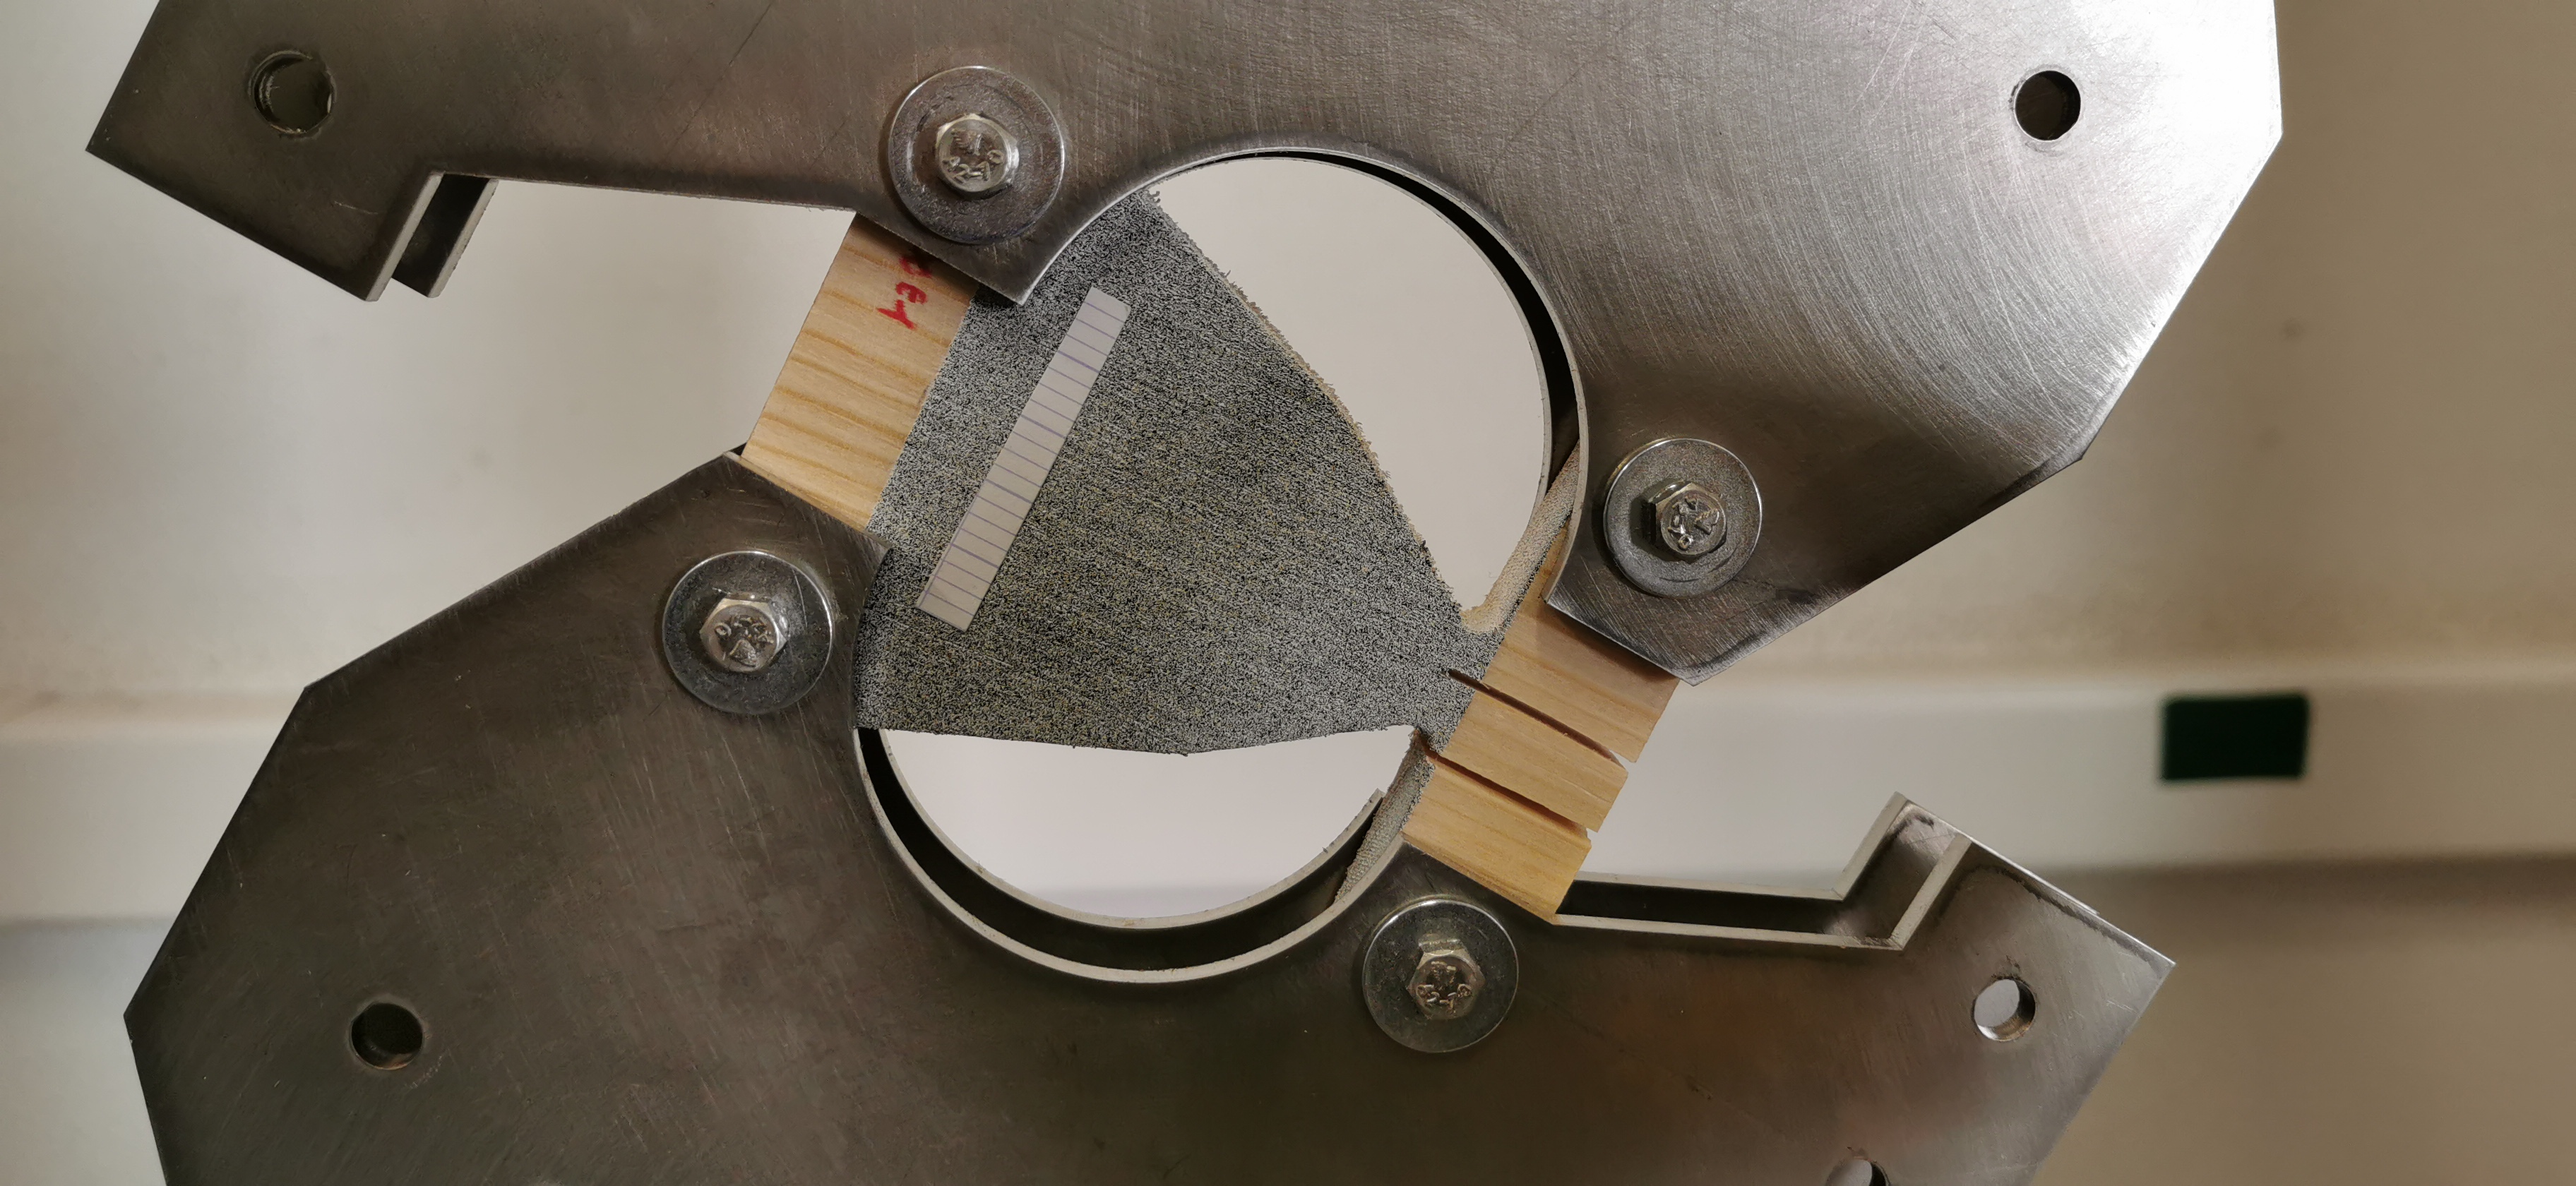
\includegraphics[width=12cm]{Crack_junction}
	\caption{Fracture issues encountered at the connection fillets}
	\label{fig:Crack_junction}
\end{figure}